\documentclass[UTF8,a4paper,autofakebold,15pt]{ctexart}

\usepackage{xeCJK}
\usepackage{fontspec}
\usepackage{ulem}
\usepackage{amsmath}
\usepackage{setspace}
\usepackage{amssymb}
\usepackage{listings}
\usepackage{titlesec}
\usepackage{multicol}
\usepackage{graphicx}
\usepackage{subfig}
\usepackage{multirow}
\usepackage[colorlinks, linkcolor=black]{hyperref}
\usepackage{geometry}
\newcommand{\ee}{\mathrm e}
\newcommand{\ii}{\mathrm i}
\usepackage{xcolor}
\lstset{
	columns=fixed, 
	tabsize=4,
	frame=none,                                          % 不显示背景边框
	numbers=left,
	backgroundcolor=\color[RGB]{245,245,244},            % 设定背景颜色
	keywordstyle=\color[RGB]{40,40,255},                 % 设定关键字颜色
	numberstyle=\footnotesize\color{darkgray},           % 设定行号格式
	commentstyle=\it\color[RGB]{0,96,96},                % 设置代码注释的格式
	basicstyle=\ttfamily,
	stringstyle=\ttfamily\slshape\color[RGB]{128,0,0},   % 设置字符串格式
	showstringspaces=false,                              % 不显示字符串中的空格
	language=verilog,                                        % 设置语言
	breaklines=true,
}
\geometry{left=3cm,right=3cm,top=2.5cm,bottom=2.0cm}

\newCJKfontfamily\sonti{STSongti-SC-Regular}[BoldFont=STSongti-SC-Bold]

\newCJKfontfamily\Sonti{STSongti-SC-Bold}[BoldFont=STSongti-SC-Bold]

\setCJKmonofont{STSongti-SC-Regular}[BoldFont=STSongti-SC-Bold]

\titleformat*{\section}{\centering\zihao{-2}\bfseries}

\titleformat*{\subsection}{\zihao{4}\bfseries}

\title{武汉大学计算机学院\\
	本科生课程设计报告
}
\author{}
\date{}
\setmainfont{Times New Roman}
\pagestyle{plain}
\begin{document}
	
	\begin{center}
		
	\vspace{50pt}
	{\zihao{1}\tt 武汉大学计算机学院\\\vspace{10pt}
		本科生课程设计报告}
	
	\vspace{50pt}
	
	{\heiti\zihao{2}\bf RISC-V CPU设计}
	
	\vspace{100pt}
	
	\begin{spacing}{1.5}
	\zihao{-3}
	\qquad\begin{tabular}{ll}
		专\ 业\ 名\ 称   :&计算机科学与技术(弘毅学堂)\\
		
		课\ 程\ 名\ 称   :&计算机系统综合设计\\
		
		指\ 导\ 教\ 师   :&内切圆\ 副教授\\
		
		学\ 生\ 学\ 号   :&2020400004071\\
		
		学\ 生\ 姓\ 名   :&外接圆
	\end{tabular}

	\end{spacing}

	\vspace{100pt}

	\zihao{3} 二〇二三年七月
	
	\end{center}
	

\newpage

	\begin{center}
	{\zihao{2}\Sonti 郑\ 重\ 声\ 明}
	\end{center}

	\vspace{40pt}
	
	\zihao{4}
	本人呈交的实验报告,是在指导老师的指导下,独立进行实验工作所取得的成果,所有数据、图片资料真实可靠。尽我所知,除文中已经注明引用的内容外,本实验报告不包含他人享有著作权的内容。对本实验报告做出贡献的其他个人和集体,均已在文中以明确的方式标明。本实验报告的知识产权归属于培养单位。
	
	\vspace{40pt}
	
	本人签名:\_\_\_\_\_\_\_\_\_\_  \qquad\qquad\qquad        日期:\_\_\_\_\_\_\_\_\_\_
	
\newpage

	\zihao{-2}
	
	\begin{center}
		{\bf 摘\quad 要}
	\end{center}
	
	\zihao{-4}
	
	本实验的实验目的是完成基于\LaTeX 的武汉大学计算机学院实验报告设计,使其支持绝大多数课程要求(要求交word的课程除外)。
	
	实验设计主要遵循【计算机组成与设计课程设计】\cite{ref1}的实验报告格式,其他课程{\bf 大同小异}。
	
	实验内容主要包括:各个标题、段落、格式的生成,并可插入代码段,本报告使用Verilog语言。
	
	实验结论为:\LaTeX 可以高度复现武汉大学(计算机学院)实验报告。
	
	仓库地址:\href{https://github.com/wjy-yy/whucs-latex}{https://github.com/wjy-yy/whucs-latex}
	
	{\bf 关键词:}武汉大学;计算机学院;\LaTeX;实验报告
	
\newpage

	\zihao{-2}
	
	\begin{center}
		{\bf 目\quad 录}
	\end{center}
	
	\zihao{-4}
	
	\renewcommand{\contentsname}{}
	
	\tableofcontents
	
\newpage


\section{引言}

\subsection{实验目的}

	{\tt section}的大标题为{\bf 黑体小二字号},{\tt subsection}的小标题为{\bf 黑体小四字号}。

\subsection{国内外研究现状}

	目前暂未发现其他仓库上传了武汉大学计算机学院实验报告 \LaTeX 模板。

\newpage

\section{实验环境介绍}

\subsection{\LaTeX}
	\LaTeX 是一个文档准备系统 (Document Preparing System),它非常适用于生成高印刷质 量的科技类和数学类文档。它也能够生成所有其他种类的文档,小到简单的信件,大到完整的书 籍。LATEX 使用 TEX [6] 作为它的排版引擎。

	使用文档参见:\href{https://texdoc.org/serve/lshort-zh-cn.pdf/0}{https://texdoc.org/serve/lshort-zh-cn.pdf/0}

\subsection{本地编译环境}

	一般macOS推荐使用 TeX Live 作为编译器,VS Code 或 TeX Studio作为编辑器。


\newpage

\section{概要设计 - 单周期}

\subsection{图片示例}

插入图片可以是pdf格式,也可以是其他各种格式,而pdf可以作为矢量插入。

\begin{figure}[ht]
	\centering
	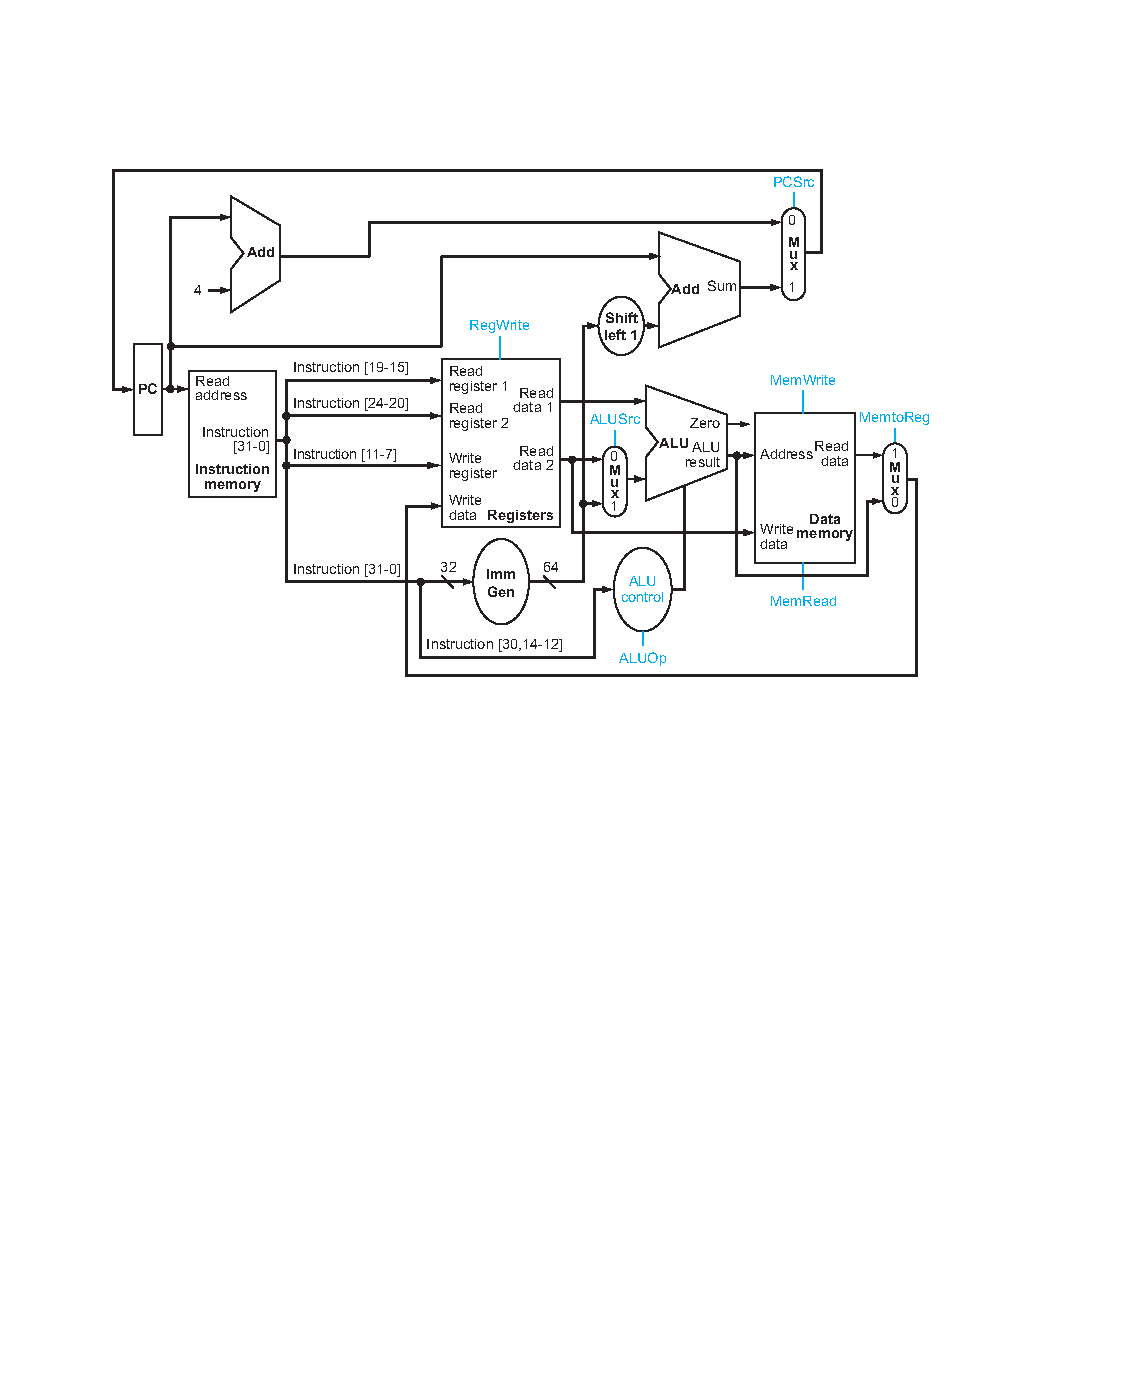
\includegraphics{fig1.pdf}
	\caption{单周期CPU概要原理图\cite{ref1}}
	\label{fig:label1}
\end{figure}

此外,{\tt ctrl\_encode\_def.v}文件进行各类控制信号和指令内容的宏定义,{\tt sccomp\_tb.v}中存放测试文件,进行仿真时的控制和调试。

\subsection{表格示例}

\subsubsection{功能描述}

	根据输入信号(包括输入数据以及控制信号)输出程序需要执行的指令地址,并向IM(指令存储器)输出这个地址。该值在每个指令周期用NPC模块的输出进行更新。

\subsubsection{模块接口}
	插入表格示例。

	\begin{center}

	\begin{tabular}{|c|c|c|}
		\hline
		信号名&方向&描述\\
		\hline
		{\tt clk}&input&时钟信号\\
		\hline
		{\tt rst}&input&复位信号\\
		\hline
		{\tt NPC}&input&来自{\tt NPC}模块的控制下一PC的输入\\
		\hline
		{\tt PC}&output&输出的PC信号\\
		\hline
	\end{tabular}

	\end{center}

\subsection{RF(寄存器文件)}

\subsubsection{功能描述}

	控制32个寄存器的读写操作。在任意时刻都可以根据输入{\tt A1[4:0]}和{\tt A2[4:0]}的值读取指定编号的寄存器的值,并赋值给{\tt RD1[31:0]},{\tt RD2[31:0]}作为输出。当时钟处在上升沿时,并且写寄存器信号{\tt RFWr}有效,由{\tt A3[4:0]}的值决定向指定编号的寄存器写入{\tt WD[31:0]}的值。

\subsubsection{模块接口}

	表略,参见{\tt mac-example/}。

\newpage
\section{详细设计 - 单周期}

\subsection{参考文献引用示例}

依据教材《计算机组成与设计:软/硬件接口 RISC-V(第五版)》\cite{ref1}中单周期架构CPU各模块的输入、输出端口,功能信号的规定以及RISC-V指令集中各个指令对应的数据周转流程与对应信号。模块中所有连线基于该架构进行实现。

\subsection{代码段插入示例}

{\tt SCPU.v}设计如下:(省略连线,详见附件中{\tt .v}文件)

{\lstset{language=verilog}\zihao{5}
\begin{lstlisting}
`include "ctrl_encode_def.v"
module SCPU(
	input      clk,          // 时钟信号
	input      reset,        // 复位信号
	input [31:0]  inst_in,   // 输入指令
	input [31:0]  Data_in,   // 来自 DM 的数据

	output    mem_w,        // DM 写使能
	output [31:0] PC_out,   // 输出 PC 地址( debug 用)

	output [31:0] Addr_out, // ALU 输出值(一般用于计算地址)
	output [31:0] Data_out, // 输入 DM 的数据
	output [2:0] DMType     // 选择访问 DM 的字节数
);
	assign Addr_out=aluout;
	assign B = (ALUSrc) ? immout : RD2; // ALU 第二个操作数的来源
	assign Data_out = RD2;
	
	assign iimm_shamt=inst_in[24:20]; //UJ 型指令
	assign iimm=inst_in[31:20];  //I 型指令
	assign simm={inst_in[31:25],inst_in[11:7]}; //S 型指令
	assign bimm={inst_in[31],inst_in[7],inst_in[30:25],inst_in[11:8]};  //SB 型
	assign uimm=inst_in[31:12];  //U 型
	assign jimm={inst_in[31],inst_in[19:12],inst_in[20],inst_in[30:21]};  //J 型
	
	assign Op = inst_in[6:0];  // opcode 部分
	assign Funct7 = inst_in[31:25]; // funct7 部分
	assign Funct3 = inst_in[14:12]; // funct3 部分
	assign rs1 = inst_in[19:15];  // rs1 序号
	assign rs2 = inst_in[24:20];  // rs2 序号
	assign rd = inst_in[11:7];  // rd 序号
	assign Imm12 = inst_in[31:20];
	assign IMM = inst_in[31:12];
	
	// 各模块的例化
	ctrl U_ctrl(.Op(Op), .Funct7(Funct7), .Funct3(Funct3), .Zero(Zero), .RegWrite(RegWrite), .MemWrite(mem_w),
		.EXTOp(EXTOp), .ALUOp(ALUOp), .NPCOp(NPCOp), 
		.ALUSrc(ALUSrc), .GPRSel(GPRSel), .WDSel(WDSel), .DMType(DMType) );
	PC U_PC(.clk(clk), .rst(reset), .NPC(NPC), .PC(PC_out) );
	NPC U_NPC(.PC(PC_out), .NPCOp(NPCOp), .IMM(immout), .NPC(NPC), .aluout(aluout) );
	EXT U_EXT(.iimm_shamt(iimm_shamt), .iimm(iimm), .simm(simm), .bimm(bimm), .uimm(uimm), .jimm(jimm),
	.EXTOp(EXTOp), .immout(immout) );
	RF U_RF(.clk(clk), .rst(reset), .RFWr(RegWrite), 
	.A1(rs1), .A2(rs2), .A3(rd), //Read1, Read2, Write
	.WD(WD), //Write data
	.RD1(RD1), .RD2(RD2) //Read1 Read2
	);
	alu U_alu(.A(RD1), .B(B), .ALUOp(ALUOp), .C(aluout), .Zero(Zero), .PC(PC_out) );
always @*
begin
	case(WDSel)
		`WDSel_FromALU: WD<=aluout;
		`WDSel_FromMEM: WD<=Data_in;
		`WDSel_FromPC: WD<=PC_out+4;
	endcase
end
endmodule
\end{lstlisting}}


\subsection{PC(程序计数器)}

代码略,参见{\tt mac-example/}。

\newpage
\section{概要设计 - 流水线}

\section{详细设计 - 流水线}

\newpage
\section{测试及结果分析}

\subsection{分栏示例(此处为代码分栏)}

\begin{multicols}{2}
{\zihao{5}
\begin{lstlisting}
addi x5, x0, 1000
addi x4, x0, 10
lui x6, 0xffff
sw x6, 4(x5)
lh x7, 4(x5)
sub x8, x7, x6
ori x9, x0, 111
andi x9, x9, 0
skip1:
xori x9, x9, 1
bne x0, x9, skip1
or x9, x4, x0
srli x10, x5, 10
skip2:
add x10, x9, x9
bge x9, x10, skip2
sw x9, 8(x5)
lw x28, 8(x5)
addi x29, x4, 0
jal x1, mut
sll x11, x10, x9
srai x14, x10, 2
sb x11 16(x5)
and x8, x7, x6
auipc x12, 4
lbu x13, 16(x5)
bgeu x8, x7, end

beq x0, x0, end

mut: #x28*x29
beq x29, x0, end4
addi x30, x0, 0
addi x31, x0, 0
loop:
add x31, x31, x28
addi x30, x30, 1
blt x30, x29, loop
end4:
jalr x0, x1, 0

end:
\end{lstlisting}}
\end{multicols}
\subsection{仿真测试结果}
\subsubsection{引用图片标号示例}

下一周期时,第6行代码仍在EX阶段,第5行代码执行WB阶段,此时MEM/WB里已有x7的值,通过旁路将其传入EX/MEM阶段即可。

{\color{red}{注意下一行“图”后面的数字可以点击。}}

如图\ref{fig:label10}为第8周期的仿真图像。

\begin{figure}
	\centering
	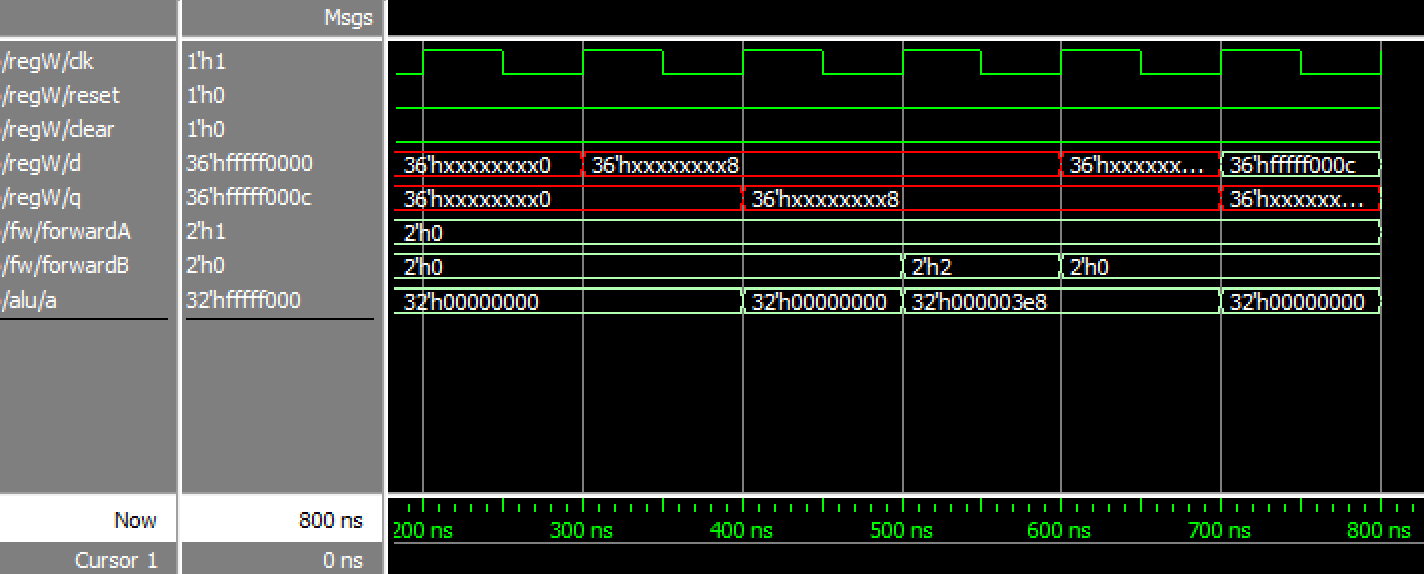
\includegraphics[scale=.8]{fig10.png}
	\caption{出现数据冒险时相关线路的仿真(第8周期)}
	\label{fig:label10}
\end{figure}

此时还没有x7的数据(0xffff0000)出现,所以无法将其前递到ALU的操作数$a$处。

\section{实验总结}
\subsection{实验总结}

本模板如对你产生帮助,请在\href{https://github.com/wjy-yy/whucs-latex}{https://github.com/wjy-yy/whucs-latex}进行star$\star$。


	
\subsection{取得的收获}
	
\newpage
\begin{thebibliography}{99}  
	
	\bibitem{ref1}David A. P, John L.H, 计算机组成与设计:硬件/软件接口[M].易江芳,刘先华.北京:机械工业出版社,2020.
	\bibitem{ref2}芮雪,王亮亮,杨琴.国产处理器研究与发展现状综述[J].现代计算机(专业版),2014(08):15-19.
	\bibitem{ref3}潘树朋,刘有耀.RISC-V微处理器以及商业IP的综述[J].单片机与嵌入式系统应用,2020,20(06):5-8+12.
	\bibitem{ref4}全球首颗智能穿戴领域人工智能芯片发布[J].智能城市,2019,5(10):191.
	\bibitem{ref5}雷思磊.RISC-V架构的开源处理器及SoC研究综述[J].单片机与嵌入式系统应用,2017,17(02):56-60+76.
	\bibitem{ref6}袁攀. 基于嵌入式RISC-V微处理器的流水线研究与设计[D].长沙理工大学,2021.DOI:10.26985/d.cnki.gcsjc.2021.000811.
	\bibitem{ref7}李亚民.计算机原理与设计:Verilog HDL版[M].北京:清华大学出版社,2011.
	
\end{thebibliography}
\newpage
\begin{center}
	\zihao{3} 教师评语评分
\end{center}

\zihao{4} \noindent 评语:\underline{\hspace{14.5cm}}

\vspace{10pt}
\underline{\hspace{15cm}}

\vspace{10pt}
\underline{\hspace{15cm}}

\vspace{10pt}
\underline{\hspace{15cm}}

\vspace{10pt}
\underline{\hspace{15cm}}

\vspace{10pt}
\underline{\hspace{15cm}}

\vspace{10pt}
\underline{\hspace{15cm}}

\vspace{10pt}
\underline{\hspace{15cm}}

\vspace{10pt}

\hspace{6cm}评阅人:\underline{\hspace{5cm}}

\hspace{9cm}年\quad\qquad 月\quad\qquad 日

\noindent\nolinebreak(备注:对该实验报告给予优点和不足的评价,并给出百分制评分。)

\end{document}